\documentclass{article}
\usepackage[utf8]{inputenc}
\usepackage{forest}
\usepackage{graphicx}
\usepackage{amsmath}
\usepackage{amssymb}
\usepackage{booktabs} % for "\midrule" macro
\usepackage{lipsum} % for filler text
\usepackage{enumerate}
\usepackage{amsmath}
\usepackage{array}
\usepackage{lplfitch}
\usepackage{hyperref}
\usepackage{caption}
\usepackage{bbm}
\usepackage{tikz}
\usetikzlibrary{automata,positioning}
\usepackage{listings}
\usepackage{color}
\usepackage{fancyhdr}
\pagestyle{fancy}
\lhead{Abanob Tawfik}
\rhead{z5075490}

\definecolor{dkgreen}{rgb}{0,0.6,0}
\definecolor{gray}{rgb}{0.5,0.5,0.5}
\definecolor{mauve}{rgb}{0.58,0,0.82}

\lstset{frame=tb,
  language=Java,
  aboveskip=3mm,
  belowskip=3mm,
  showstringspaces=false,
  columns=flexible,
  basicstyle={\small\ttfamily},
  numbers=none,
  numberstyle=\tiny\color{gray},
  keywordstyle=\color{blue},
  commentstyle=\color{dkgreen},
  stringstyle=\color{mauve},
  breaklines=true,
  breakatwhitespace=true,
  tabsize=3
}
%note this LaTeX package was not written by me and taken from stackexchange forums to be used to write java code formatted
%link to original page https://stackoverflow.com/questions/3175105/inserting-code-in-this-latex-document-with-indentation
%%%%%%%%%%%%%%%%%%%%%%%%%%%%%%%%%%%%%%%%%%%%%%%%%%%%%%%%%%%%%%%%%%%%%%%%%%%%%%%%%%%%%%%%%%%%%
\usepackage{listings}
\usepackage{color}
\newcommand*\fixindent{ \hspace{1pt}\\}
\newcommand{\squeezeup}{\vspace{-2.5mm}}




\title{comp3411 assignment 2}
\author{Abanob Tawfik\\z5075490\\z5075490@student.unsw.edu.au }
\date{April 2020}

\begin{document}
\maketitle
\section{Decision trees}

Consider the decision tree learning algorithm of Figure 7.7 and the data of Figure 7.1
from Poole \& Mackworth [1], also presented below. Suppose, for this question, the
stopping criterion is that all of the examples have the same classification. The tree of
Figure 7.6 was built by selecting a feature that gives the maximum information gain.
This question considers what happens when a different feature is selected.

\begin{center}
\hspace*{1pt}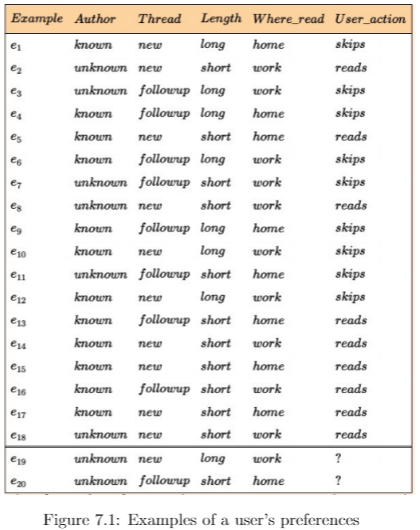
\includegraphics[width=250px,height=290px]{dataa.png}
\end{center}

\newpage
\begin{center}
\hspace*{1pt}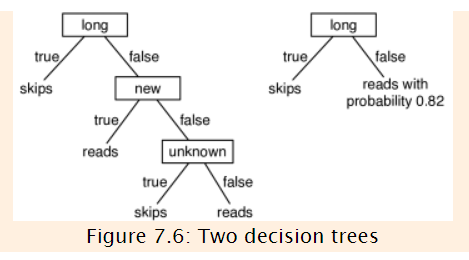
\includegraphics{treeeeee.png}
\end{center}
For the following Question the if then else statements representing the decision tree found with the maximum information gain split is given below.\\
\begin{lstlisting}
    if(e.Length == short){
        if(e.Thread == new){
            return "Read";
        }
        else{
            if(e.Author == known){
                return "Read";
            }
            else{
                return "Skip";
            }
        }
    }
    else{
        return "Skip";
    }
\end{lstlisting}
\fixindent{}\fixindent{}\fixindent{}\fixindent{}\fixindent{}\fixindent{}\fixindent{}
\begin{enumerate}[(a)]
    \item \textbf{Suppose you change the algorithm to always select the first element of the list of features. What tree is found when the features are in the order [\emph{Author, Thread, Length, WhereRead}]? Does this tree represent a different function than that found with the maximum information gain split? Explain.}\\Solution:\\
    The following decision tree is made by selecting attributes in the order; Author, Thread, Length and WhereRead
    \begin{center}
\hspace*{-2cm} 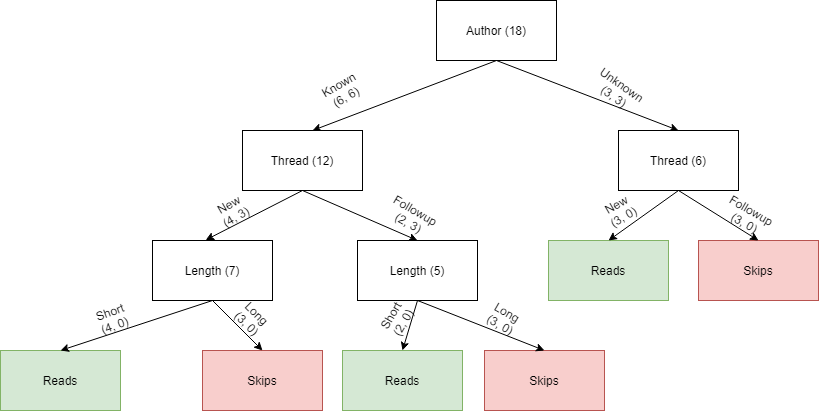
\includegraphics[width=425px,height=220px]{tree1.png}
    \end{center}\\
    This decision tree represents a different function than the tree from Figure 7.6 with the maximum information gain splits. The following if then else statements on the next page represent the function of the tree.\\ 
    \newpage
        \begin{lstlisting}
            if(e.author == known){
                if(e.Thread == new){
                    if(e.Length == short){
                        return "Read";
                    }
                    else{
                        return "Skip";
                    }
                }
                else{
                    if(e.Length == short){
                        return "Read";
                    }
                    else{
                        return "Skip";
                    }
                }
            }
            else{
                if(e.Thread == new){
                    return "Read";
                }
                else{
                    return "Skip";
                }
            }
        \end{lstlisting}
        As can been seen from the following flow of the functions, when classifying example 19 [\emph{unknown, new, long, reads}] the maximum information split tree gives us "Skip" as the output, as the first branch of the tree will give us "skip" since the example has length "long". With the decision tree we created example 19 gives us "read" as the output. when we follow the tree, since the author is unknown and the thread is new, the tree chooses "read". In the tree we created, the length of the article is irrelevant when the author is unknown, whereas in the maximum information split tree, length is the initial decider.
        \newpage
    \item \textbf{What tree is found when the features are in the order [\emph{WhereRead,Thread,Length, Author}]? Does this tree represent a different function than that found with the maximum information gain split or the one given for the preceding part? Explain.} \\Solution:\\
    The following decision tree is made by selecting attributes in the order; WhereRead, Thread, Length and Author
    \begin{center}
    \hspace*{-3cm} 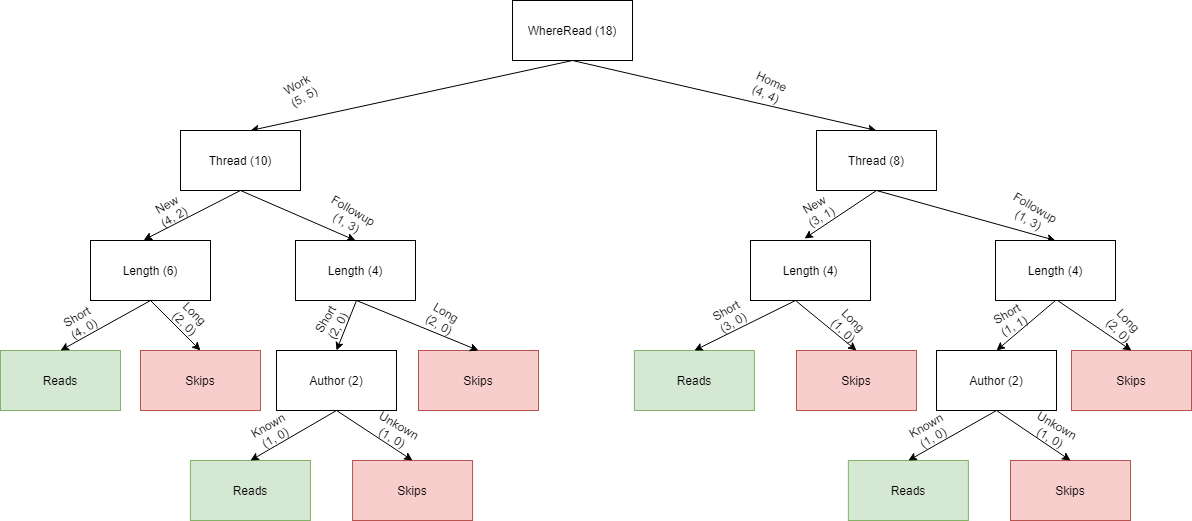
\includegraphics[width=475px,height=250px]{tree2.png}
    \end{center}\\
    This decision tree represents the same function as the tree from Figure 7.6 with the maximum information gain splits. The following if then else statements on the next page represent the function of the tree.
    \newpage
    \begin{lstlisting}
        if(e.WhereRead == Work){
            if(e.Thread == New){
                if(e.Length == Short){
                    return "Read";
                }
                else{
                    return "Skip";
                }
            }
            else{
                if(e.Length == Short){
                    if(e.Author == Known){
                        return "Read";
                    }
                    else{
                        return "Skip";
                    }
                }
                else{
                    return "Skip";
                }
            }
        }
        else{
            if(e.Thread == New){
                if(e.Length == Short){
                    return "Read";
                }
                else{
                    return "Skip";
                }
            }
            else{
                if(e.Length == Short){
                    if(e.Author == Known){
                        return "Read";
                    }
                    else{
                        return "Skip";
                    }
                }
                else{
                    return "Skip";
                }
            }
        }
    \end{lstlisting}\fixindent{}
The following tree represents the same function as the tree created with the maximum information gain split. Upon using both trees for classification on the test examples, they both had come to the same outcome, E18 was skip as on both trees, anytime length appeared as a node, the Long branch was always Skip. E19 had also turned into skip despite being short, as unknown  followups had also ended up being leaves for skip. By comparing the features on both trees we can see that both trees will behave the same for all the same features.\\

Length: All Long articles skip, as each long transition has a leaf node for skip. All short articles are read provided either the thread is new, or the thread is a followup but the author is known. This can be seen also in the maximum information gain tree.\\

Thread: All follow up threads were only read provided they are short and the author is known. all new threads will be read provided the article is short. This can be seen also in the maximum information gain tree.\\

WhereRead: Regardless of the value of WhereRead, the output was not effected, this can be seen similair to above, where the children of WhereRead are identical, and the maximum information gain tree did not contain a node for WhereRead as it has no impact.\\

Author: all unknown authors are only read provided the article is short and new. All known authors are read provided the article is short. This can be seen in both trees by comparing the paths taken to the leaves.\\

By comparing the paths taken to reach the leaves, we can see that for each input, we will have the same output for both trees, the path on the maximum information gain tree is just shorter. Since all input produce the same output for both functions, we can say both trees represent the same function. Despite the two trees representing the same function, The maximum information gain tree is far more efficient as there is alot less branches and it is much more compact. In practice whilst both produce the same output, the tree from the maximum information gain is more desirable due to its compactness and speed in practice. \\

As discussed in Part (a) we learnt that the maximum information gain tree had represented a different function than that of the tree in Part (a). From this we can say that since the tree we have found represents the same function as the one from the maximum information gain tree, and the maximum information gain tree represents a different function than the tree in Part (a), we can say that the tree we have found represents a different function than the tree in Part (a).
\newpage
\item \textbf{Is there a tree that correctly classifies the training examples but represents a different function than those found by the preceding algorithms? If so, give it. If not, explain why.}\\Solution:\\
as discussed in Part (b) the attribute WhereRead has no impact on the function of the tree. This means that the only attribute ordering which creates new trees are for the attributes [\emph{Author, Thread, Length}]. We have already discussed the tree for picking attributes in the order [\emph{Author, Thread, Length}], [\emph{Length, Thread, Author}] and [\emph{Thread, Length Author}] if  we ignore the WhereRead attribute, This means there are only three other possible ways we can choose our attribute order.
    \begin{enumerate}[(1)]
        \item{[\emph{Length, Author, Thread}]}
        \item{[\emph{Author, Length, Thread}]}
        \item{[\emph{Thread, Author, Length}]}
    \end{enumerate}
The tree from picking attributes in order (1) is the following tree below
\begin{center}
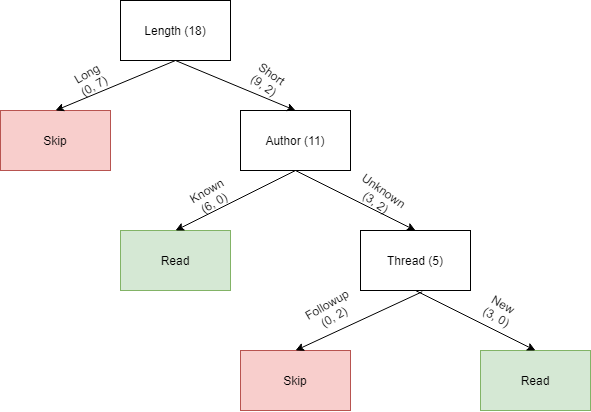
\includegraphics[width=300px,height=200px]{tree3.png}
\end{center}\\
What can be observed from the tree, is that it is the exact same tree as the maximum information gain tree By comparing the impact on each feature we see that for the  tree generated, all long articles are skipped and all short articles are read unless the author is unknown and the thread is a followup, This means that tree (1) represents the same function as the maximum information gain tree and the tree in Part (b).\\
\newpage
The tree from picking attributes in order (2) is the following tree below
\begin{center}
\hspace*{-1cm}
\includegraphics[width=376px,height=210px]{tree4.png}
\end{center}\\
What can be observed from the tree, is that the tree represents the same function as the maximum information gain tree. By comparing the impact on each feature we see that for the  tree generated, all long articles are skipped and all short articles are read unless the author is unknown and the thread is a followup. This is the exact behaviour shown in the minimal information gain tree.\newpage
The tree from picking attributes in order (3) is the following tree below
\begin{center}
\hspace*{-1cm}
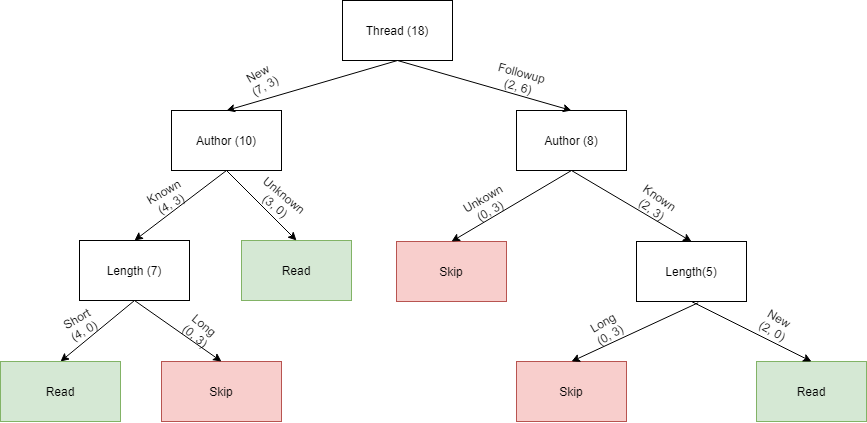
\includegraphics[width=376px,height=210px]{tree5.png}
\end{center}\\
The following tree represents a different function to the  maximum information gain tree, when comparing the impact on the features, any new thread from a unknown author will be read, even if it's length is long, whereas in the maximum information gain tree we skip all long articles. However what can be observed is that this tree represents the same function as the tree in Part (a). The tree itself is almost identical to the tree in Part (a) with Author and Thread swapped around, however what we can observe is that all feature input will have the same behaviour for both trees.

Length: Skip all long articles except for articles from unknown authors in a new thread. Read all short articles from known authors, and length has no impact on unknown authors. This is the same behaviour as seen from the tree in Part (a).\\

Thread: Read all new articles from any author provided they are not long, if the author is unknown, and the thread is new we read it otherwise we skip the article. if the author is known then Thread has no impact, as for known authors the deciding factor is the length of the article. This behaviour can be seen from the tree in Part (a) by comparing the children of known and unknown authors, and what can be observed is identical behaviour.\\

Author: For unknown authors, the deciding factor relied on only the thread value, for known authors the length of the article became the determining factor. This can be seen from the tree in Part (a) by comparing the children of known and unknown authors, drawing the same conclusions.\\

As can be seen Tree (3) represents the same function as the tree discovered in Part (a), in fact they both carry the same size and will have almost the same efficiency depending on the data received.

In conclusion we explored every possible tree that can be created by selecting attributes in all possible orders (ignoring WhereRead) and what was determined was that the trees in Part (a) and Part (b) represent all possible functions to classify the examples. This is because, WhereRead has no impact on the outcome of user action, and when we look at all remaining features, there are only three. By exhausting all possible orders to select features, all 6 combinations had simplified to the same two functions in Part (a) and Part (b).Thus there is no other tree that correctly classifies the training examples and represents a different function than that in Part (a) and Part (b).
\end{enumerate}

\newpage
\section{Decision trees}
The goal is to take out-of-the-box models and apply them to a given dataset. The task is to analyse the data and build a model to predict whether income exceeds \$50K/yr based on census data (also known as "Census Income" dataset). Use the data set Adult Data Set from the Machine Learning repository [2]. Use the supervised learning methods discussed in the lectures, Decision Trees.

\begin{flushleft}
Do not code these methods: instead use the implementations from scikit-learn. Read the scikit-learn documentation on Decision Trees [3], and the linked pages describing the parameters of the methods.\\\\
\end{flushleft}
This question will help you master the workflow of model building. For example, you’ll get to practice how to use the critical steps:

\begin{itemize}
    \item {Importing data}
    \item {Cleaning data}
    \item {Splitting it into train/test or cross-validation sets}
    \item {Pre-processing}
    \item {Transformation}
    \item {Feature engineering}
\end{itemize}
Use the sklearn documentation pages for instructions. You should need the classification algorithms.\\\\
There are also available Tutorials:
\begin{itemize}
    \item Sklearn – official tutorial for the sklearn package 
    \item Predicting wine quality with scikit-learn – Step-by-step tutorial for training a machine learning model
\end{itemize}
The data is available here: \href{http://archive.ics.uci.edu/ml/machine-learning-databases/adult/}{http://archive.ics.uci.edu/ml/machine-learning-databases/adult/}
\newpage
\fixindent{}From completing this question there were many things which i had learnt to building a model. from each critical step here is what i had done.\\
\begin{itemize}
    \item \textbf{Importing data}\\
    Using the pandas library, i had imported all the data from the files into an array of objects containing one entry for each line in the data file.
    \item \textbf{Cleaning data}\\
    Some entries contained missing fields with the '?' as their value. These entries are unable to be analysed and were removed. To do this, I had first converted all the '?' values into NaN using numpy, and then i had used the pandas dropna function to remove all entries with any field containing NaN.
    \item \textbf{Splitting into training/test data sets}\\
    This was fairly simple as there were already separate files that contained a training set and a test set. I had functionised the data retrieval process and ran it on both separate files. In the case where we only had one data set, sklearn offers a test training split module which will take a percentage section for training and a percentage section for testing and provide two different data sets from one. This was however not necessary since we had both sets separately provided to us.
    \item \textbf{Pre-processing}\\
    Some attributes were strings, and this can be problematic for creating a decision tree of large scale, and the scikit library requires all input to be enumerated int32 values. To process the data to be used in an efficient manner, i had used the label encoder provided by scikit, which enumerates the string values into int32 values for usage in their classifier.
    \item \textbf{Transformation}\\
    After cleaning and pre-processing our data, our data was in a state where it could be used in an efficient manner. By removing all garbage entries and simplifying non-integer attributes, we had an efficient model which could be used inside our decision tree.
    \item \textbf{Feature Engineering}\\
    The methods chosen for selecting features is often the make or break for a machine learning project. The two methods for selecting features offered by scikit were "gini" and "entropy". I had chosen to use entropy as the lectures had discussed entropy and i was familiar with the concept. by using entropy maximum information gain to pick attributes, we had chosen the attribute with the lowest entropy value, giving us more meaningful splits. The difference between "gini" and "entropy" were very minor when it came to the accuracy of the classifier. When selecting a maximum depth for the tree in the classifier, I had observed that depths greater than 6 produced almost no increased accuracy, and depths of around 30 had lower accuracy, this can be attributed to Occham's Razor and overfitting. In order to pick a more generalised and readable tree, I had chosen my maximum feature depth as 6.
\end{itemize}
Below will show the code used in the creation of this project.

\begin{center}
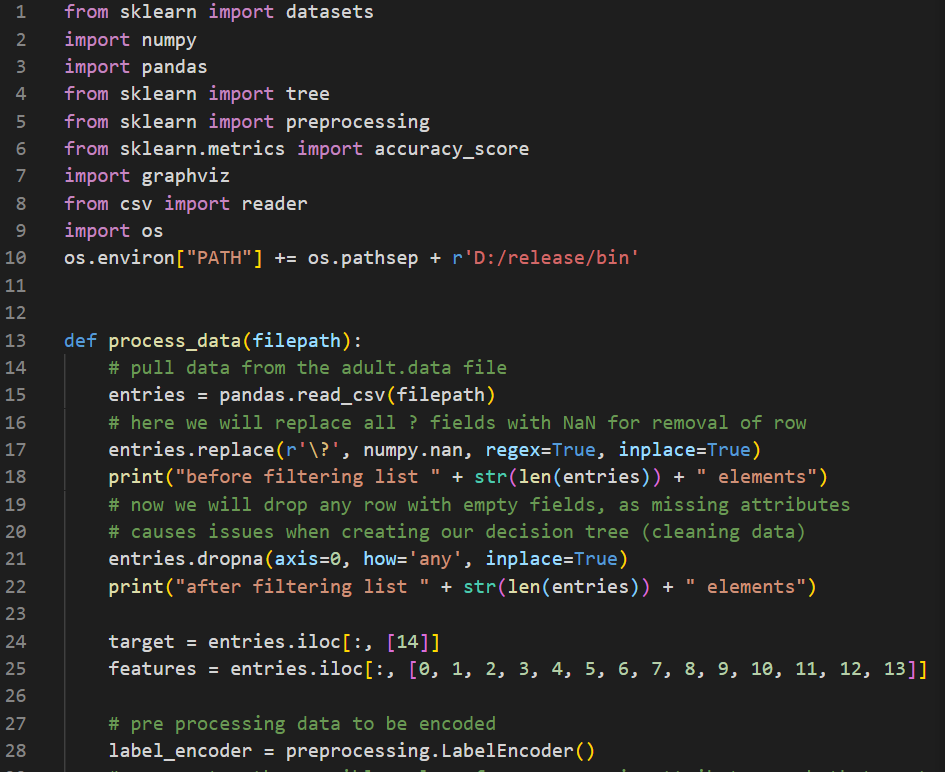
\includegraphics[width=400px,height=250px]{Screenshot_1.png}
\end{center}

\begin{center}
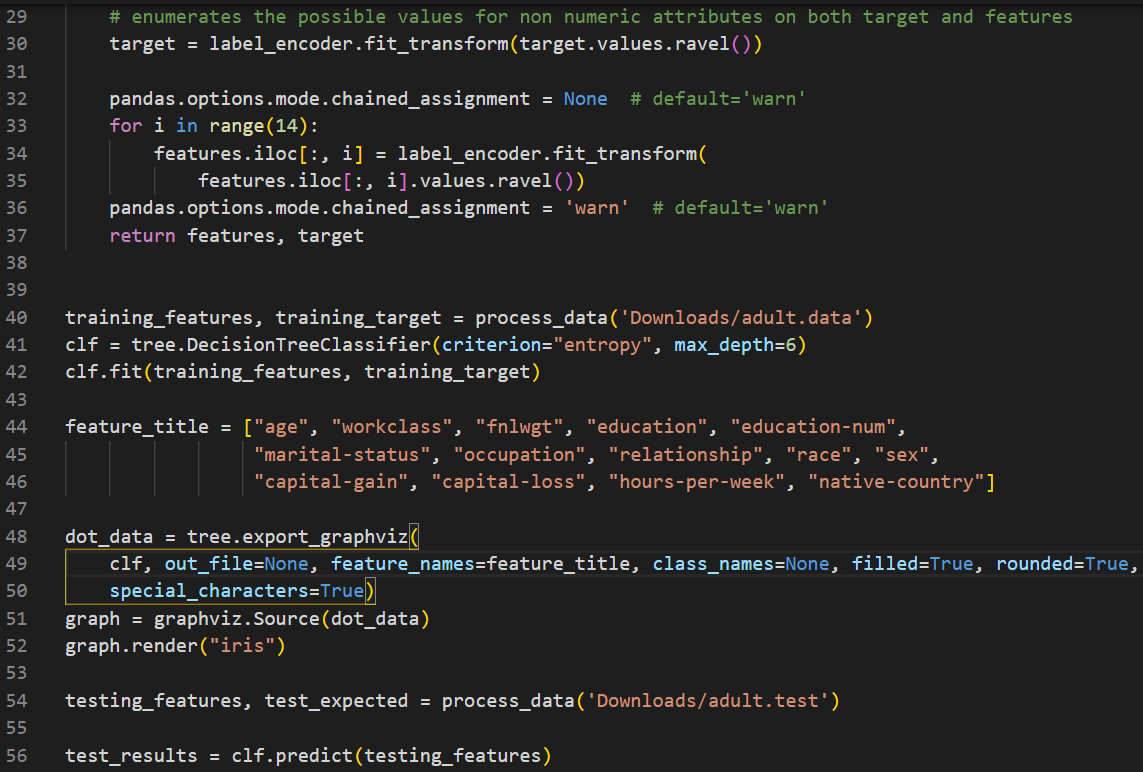
\includegraphics[width=400px,height=250px]{Screenshot_2.png}
\end{center}

\begin{center}
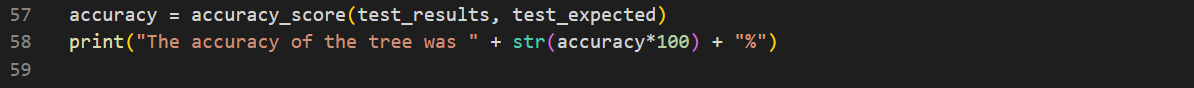
\includegraphics[width=400px,height=50px]{Screenshot_3.png}
\end{center}
\\
Output of the code shown below
\begin{center}
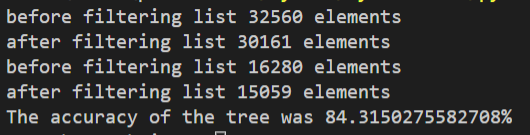
\includegraphics[width=400px,height=90px]{Screenshot_4.png}
\end{center}\\
The next page shows the decision tree that was created for the classifier using the methods described previously. If the image is too difficult to read, a link is provided below to the full decision tree pdf file, you can zoom in to take a more detailed view.\\
\href{https://documentcloud.adobe.com/link/track?uri=urn\%3Aaaid\%3Ascds\%3AUS\%3A613d445e-e5bb-4fe5-a9d2-94f948ea9746}{https://documentcloud.adobe.com/link/track?uri=urn\%3Aaaid\%3Ascds\%3AUS\%3A613d445e-e5bb-4fe5-a9d2-94f948ea9746}
\end{document}
